\PassOptionsToPackage{unicode=true}{hyperref} % options for packages loaded elsewhere
\PassOptionsToPackage{hyphens}{url}
%
\documentclass[]{article}
\usepackage{lmodern}
\usepackage{amssymb,amsmath}
\usepackage{ifxetex,ifluatex}
\usepackage{fixltx2e} % provides \textsubscript
\ifnum 0\ifxetex 1\fi\ifluatex 1\fi=0 % if pdftex
  \usepackage[T1]{fontenc}
  \usepackage[utf8]{inputenc}
  \usepackage{textcomp} % provides euro and other symbols
\else % if luatex or xelatex
  \usepackage{unicode-math}
  \defaultfontfeatures{Ligatures=TeX,Scale=MatchLowercase}
\fi
% use upquote if available, for straight quotes in verbatim environments
\IfFileExists{upquote.sty}{\usepackage{upquote}}{}
% use microtype if available
\IfFileExists{microtype.sty}{%
\usepackage[]{microtype}
\UseMicrotypeSet[protrusion]{basicmath} % disable protrusion for tt fonts
}{}
\IfFileExists{parskip.sty}{%
\usepackage{parskip}
}{% else
\setlength{\parindent}{0pt}
\setlength{\parskip}{6pt plus 2pt minus 1pt}
}
\usepackage{hyperref}
\hypersetup{
            pdftitle={Choosers: The design and evaluation of a visual algorithmic music composition language for non-programmers},
            pdfauthor={Matt Bellingham; Simon Holland; Paul Mulholland},
            pdfborder={0 0 0},
            breaklinks=true}
\urlstyle{same}  % don't use monospace font for urls
\usepackage{graphicx,grffile}
\makeatletter
\def\maxwidth{\ifdim\Gin@nat@width>\linewidth\linewidth\else\Gin@nat@width\fi}
\def\maxheight{\ifdim\Gin@nat@height>\textheight\textheight\else\Gin@nat@height\fi}
\makeatother
% Scale images if necessary, so that they will not overflow the page
% margins by default, and it is still possible to overwrite the defaults
% using explicit options in \includegraphics[width, height, ...]{}
\setkeys{Gin}{width=\maxwidth,height=\maxheight,keepaspectratio}
\setlength{\emergencystretch}{3em}  % prevent overfull lines
\providecommand{\tightlist}{%
  \setlength{\itemsep}{0pt}\setlength{\parskip}{0pt}}
\setcounter{secnumdepth}{5}
% Redefines (sub)paragraphs to behave more like sections
\ifx\paragraph\undefined\else
\let\oldparagraph\paragraph
\renewcommand{\paragraph}[1]{\oldparagraph{#1}\mbox{}}
\fi
\ifx\subparagraph\undefined\else
\let\oldsubparagraph\subparagraph
\renewcommand{\subparagraph}[1]{\oldsubparagraph{#1}\mbox{}}
\fi

% set default figure placement to htbp
\makeatletter
\def\fps@figure{htbp}
\makeatother


\title{Choosers: The design and evaluation of a visual algorithmic music
composition language for non-programmers}
\author{Matt Bellingham \and Simon Holland \and Paul Mulholland}
\date{PPIG 2018}

\begin{document}
\maketitle
\begin{abstract}
Algorithmic music composition involves specifying music in such a way
that it is non-deterministic on playback, leading to music which has the
potential to be different each time it is played. Current systems for
algorithmic music composition typically require the user to have
considerable programming skill and may require formal knowledge of
music. However, much of the potential user population are music
producers and musicians (some professional, but many amateur) with
little or no programming experience and few formal musical skills. To
investigate how this gap between tools and potential users might be
better bridged we designed Choosers, a prototype algorithmic programming
system centred around a new abstraction (of the same name) designed to
allow non-programmers access to algorithmic music composition methods.
Choosers provides a graphical notation that allows structural elements
of key importance in algorithmic composition (such as sequencing,
choice, multi-choice, weighting, looping and nesting) to be foregrounded
in the notation in a way that is accessible to non-programmers. In order
to test design assumptions a Wizard of Oz study was conducted in which
seven pairs of undergraduate Music Technology students used Choosers to
carry out a range of rudimentary algorithmic composition tasks. Feedback
was gathered using the Programming Walkthrough method. All users were
familiar with Digital Audio Workstations, and as a result they came with
some relevant understanding, but also with some expectations that were
not appropriate for algorithmic music work. Users were able to
successfully make use of the mechanisms for choice, multi-choice,
looping, and weighting after a brief training period. The `stop'
behaviour was not so easily understood and required additional input
before users fully grasped it. Some users wanted an easier way to
override algorithmic choices. These findings have been used to further
refine the design of Choosers.
\end{abstract}

\hypertarget{introduction}{%
\section{Introduction}\label{introduction}}

Algorithmic composition typically involves structural elements such as
indeterminism, parallelism, choice, multi-choice, recursion, weighting,
and looping {[}@Jacob1996-zf{]}. There are powerful existing tools, such
as Max {[}@Puckette1991-vy{]} and SuperCollider {[}@McCartney2002-uz{]}
for manipulating these and other elements of music. However, while these
systems give great compositional power to musicians who are also skilled
programmers {[}@Wilson2011-pu{]}, many musicians who are not also expert
programmers find these tools inaccessible and difficult to understand
and use {[}@Bullock2011-sw{]}.

This paper presents an evaluation of a prototype visual programming
language {[}@Bellingham2017-qb{]} designed to allow structural elements
of the kind involved in algorithmic music composition to be readily
visualised and manipulated, while making little or no demand on
programming ability. This system, called Choosers, centres around a
novel non-standard programming abstraction (the Chooser) which controls
indeterminism, parallelism, choice, multi-choice, recursion, weighting,
and looping.

In this paper we present a programming walkthrough evaluation carried
out with seven pairs of undergraduate Music Technology students. The
purpose of this evaluation is to:

\begin{itemize}
\tightlist
\item
  Test the ability of self-taught music producers without programming
  skills to use Choosers to carry out a range of rudimentary algorithmic
  composition tasks;
\item
  Identify usability and user experience problems in the current design;
\item
  Identify tensions and trade-offs in the interaction design of the
  system.
\end{itemize}

In the evaluation, pairs of participants were introduced to each element
of the graphical programming language via short tutorial videos.
Participants were given a range of practical tasks to complete on paper
or a whiteboard. The facilitator played a Wizard of Oz role, rapidly
translating participants' graphical solutions into runnable code that
was fed into a non-graphical prototype version of Choosers so that
participants could hear the musical results of their attempts.

\hypertarget{related-workproblem-setting}{%
\section{Related work/problem
setting}\label{related-workproblem-setting}}

Various music programming languages are capable of algorithmic
composition, although they require significant programming skills
{[}@Bullock2011-sw{]} and are therefore inaccessible to many users.
@Bellingham2014-hf used the Cognitive Dimensions of Notations framework
{[}@Green1996-gb{]} to review the usability of a representative
selection of software capable of algorithmic music composition. The
findings of the review included the following. First, we found that most
existing software requires the user to have a considerable understanding
of constructs in either graphical (e.g Max, Pure Data) or text-oriented
(e.g.~SuperCollider, ChucK, Csound) programming languages: such
knowledge requires a significant learning overhead. Second, users are
often required to have an understanding of musical notation and/or music
production equipment such as mixing desks and patchbays. Third, several
programs imposed working practices unconducive to compositional
processes. Fourth, in some cases the user was unable to define, and
subsequently change, the musical structure. Finally, complex visual
design in graphical programming languages led to patches with multiple
connections, making them difficult to read and to navigate.

\hypertarget{sec:system}{%
\section{Introduction to the system: Choosers}\label{sec:system}}

The following section provides a brief overview of Choosers, designed to
cover enough detail to allow readers to understand the evaluation. Full
details of the system design can be found in @Bellingham2017-qb. The
system has general musical expressivity, but for simplicity the present
evaluation focuses on the manipulation of samples for algorithmic
composition.

\textbf{Samples} are shown in boxes, and can be auditioned by clicking
on them. Samples can be assembled into \textbf{sequences} using arrows
(see @fig:one). Samples in a sequence play in the order indicated by the
direction of the arrows. Only a single arrow can enter or exit each
element in a sequence. This deliberate limitation reflects the fact that
parallelism and choice are dealt with elsewhere in the language. Boxes
and sequences can be put inside other boxes, thereby packaging them into
a single unit.

\begin{figure}
\hypertarget{fig:one}{%
\centering
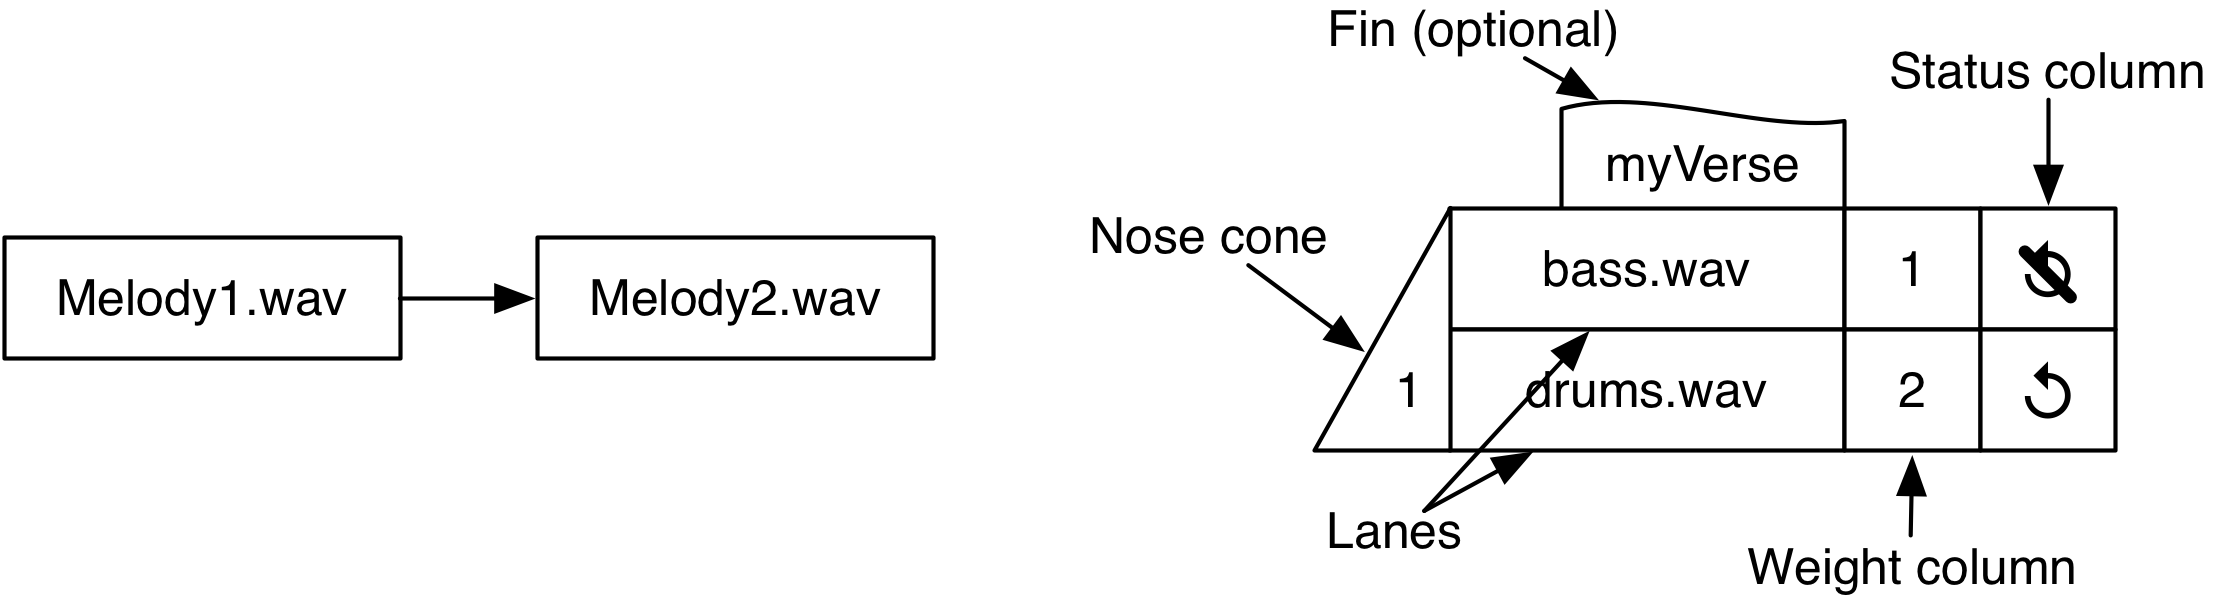
\includegraphics{./media/image1.png}
\caption{Samples are shown in boxes, and a sequence is assembled via
arrows (left); an annotated Soundable Chooser (right).}\label{fig:one}
}
\end{figure}

Boxes referring to samples or sequences can be snapped together
vertically to create what are known as \textbf{Choosers}. @Fig:one shows
a Chooser with two lanes, each containing a sample (drums and bass). The
number 1 in the nose cone indicates that at run time, just one of the
lanes will be selected at random (subject to restrictions described
below). By manipulating the number in the nose cone, any number of lanes
from 0 to 2 can be chosen randomly to play simultaneously. A Chooser can
have any number \emph{n} of lanes. By manipulating the number in the
nose cone, any number of lanes from 0 to \emph{n} can be chosen randomly
at run time and played simultaneously. Each lane has a weight associated
with it. Consequently, in @fig:one, the drums are twice as likely to be
chosen as the bass. Additionally, a weight of `A' (`always play') can be
used to ensure that the lane is always selected for playback.

Any sample can be set to \textbf{loop} indefinitely when selected on a
particular run, or to play just once by the choice indicated in the
status column (shown in @fig:one): indefinite looping of a single sample
is typically not desired, so we now introduce \textbf{Time Choosers}
(see @fig:two, left).

\begin{figure}
\hypertarget{fig:two}{%
\centering
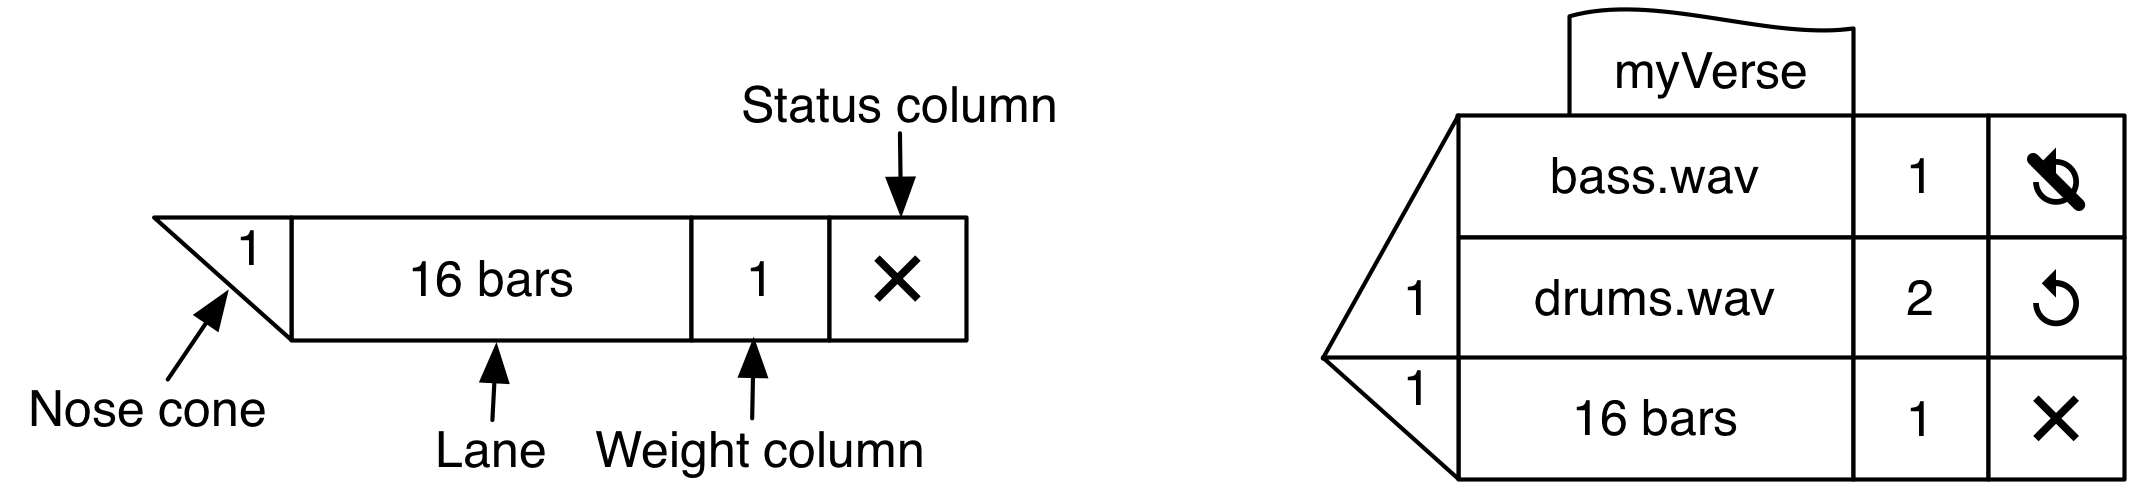
\includegraphics{./media/image2.png}
\caption{An annotated Time Chooser (left); a Full Chooser
(right).}\label{fig:two}
}
\end{figure}

If the Time Chooser (@fig:two, left) is attached to the bottom of the
Chooser (@fig:one, right) this produces a \textbf{Full Chooser}
(@fig:two, right). When the Full Chooser shown in fig.~2 is played,
looped drums, if chosen, cannot play indefinitely, but will be cut off
after 16 bars. However, if the status column in the time chooser were
set to \(>\) (indicating a \textbf{soft stop}) rather than \(\times\)
(indicating a \textbf{hard stop}) then, after 16 bars, the sample would
play to the end of its current iteration. With a hard stop, if the Time
Chooser duration cleanly divides the sample duration, every repetition
will play in full. If not (e.g.~if the bass.wav sample in fig.~2 had a
duration of 3 bars) a hard stop will cut playback mid-sample. The two
kinds of stop work similarly with non-looped lanes. If the non-looped
bass lane of the Full Chooser (@fig:two, right) were chosen, the bass
sample would be guaranteed to start playing once. With either kind of
stop, if the sample were \emph{less} than 16 bars long, there would be
silence after completion until the end of the 16 bars. A non-looped
sample longer than 16 bars would be truncated by a hard stop but allowed
to complete by a soft stop.

Now that Time Choosers and Full Choosers have been introduced, in order
to avoid ambiguity, we will refer to Choosers with no attached Time
Choosers, such as those shown in @fig:one, as \textbf{Soundable
Choosers}.

A Time Chooser can be used alone as part of a sequence -- however, when
used in this way it will simply result in a \textbf{rest} of the
specified duration. More generally, the purpose of a Time Chooser within
a Full Chooser is to moderate in a non-deterministic manner how long the
Soundable Chooser and its individual lanes play. Possible interactions
between the settings of soundable and Time Choosers can make the results
more varied than might be imagined. A Time Chooser's nose cone can be
set to either one or zero. If set to one, one time lane will be chosen
at run time. If it is set to zero no time lanes will be selected and the
Soundable Chooser will run as though there is no Time Chooser. This
allows for quick low viscosity {[}@Green1996-gb{]} arrangement changes,
with the possibility of infinite playback if the Soundable Chooser lanes
are set to loop. With no Time Chooser and the chosen lanes \emph{not}
set to loop, the samples will play and the Chooser will be released when
they have finished playing, regardless of length.

\hypertarget{method}{%
\section{Method}\label{method}}

\hypertarget{participants}{%
\subsection{Participants}\label{participants}}

Seven pairs of undergraduate Music Technology students took part in user
tests utilising a Wizard of Oz prototyping methodology. These users were
targeted as they are typically lack programming skill and extensive
formal music training. While they may be conversant with some elements
of music theory, the predominant background is self-taught music
producers with experience of making music electronically using Digital
Audio Workstations (DAWs).

All participants were asked to complete a short questionnaire before
taking part in the user tests. Of the fourteen participants all
considered themselves musicians. Six participants did not read any music
notation (though ten had some formal musical training). Most of the
music readers could read common music notation as well as chord
notation. All participants were familiar with DAWs, with Logic Pro
(Apple Inc., 2013) mentioned by all fourteen users. Other DAWs mentioned
included Pro Tools (6 mentions), Cubase (2 mentions), FL Studio (5
mentions), Reason (1 mention), and Ableton Live (1 mention). Pure Data
{[}@Puckette1991-vy{]} a visual audio programming language, was
mentioned by two participants. Twelve participants had experience using
hardware for music performance HCI tasks (such as drum pads or control
surfaces). The participants were not habitual performers; seven of the
fourteen participants do not perform with or for others. Of those that
do, three perform in church, and four occasionally play with friends in
private. Five of the fourteen participants claimed some experience in
computer programming; however, two of these considered markup for the
web (HTML and CSS) as programming. If simple markup and layout are
excluded, then more than two thirds of participants (11 out of 14) lack
experience of writing algorithms in any programming language. One
participant listed the use of Pure Data and SuperCollider. Eight of the
fourteen participants did not know what algorithmic music was at the
start of the user tests. The remaining six participants felt that they
knew what algorithmic music was but had not created any.

\hypertarget{walkthrough-protocol}{%
\subsection{Walkthrough protocol}\label{walkthrough-protocol}}

Participants were asked to take part in eight scenarios, as reproduced
below. The users were free to discuss the work and to ask for
clarification with the administrator of the test. Users were asked to
act as active participants in the research, and to help in categorising
any issues that were raised. The categorisations that users were asked
to use -- taken from the programming walkthrough method {[}@Bell1991-uw;
@Bell1992-cn{]} -- were questions (e.g.~why does the loop do that?),
problems (e.g.~I don't understand what these lanes are for), suggestions
(e.g.~maybe the cone should be a different shape), and other
observations (e.g.~I like the fins). In addition, participants were
asked if they could think of any other ways in which each scenario could
be completed. This prompted a discussion on alternative routes in order
to test understanding and to capture user expectations.

\hypertarget{walkthrough-scenarios}{%
\subsection{Walkthrough scenarios}\label{walkthrough-scenarios}}

The eight scenarios issued as part of the user tests are shown in
@fig:three. The users were introduced to each element of the graphical
programming language via short tutorial videos\footnote{Available at
  \url{https://goo.gl/PFeAJf}.}. Users were given a range of practical
tasks to complete on paper or on a whiteboard (see @fig:four), and their
outputs were played by the facilitator using a set of SuperCollider
{[}@McCartney2002-uz{]} classes written to implement the musical
abstractions behind the system. The user tests were videoed and
transcribed to assist in the analysis presented here.

\begin{figure}
\hypertarget{fig:three}{%
\centering
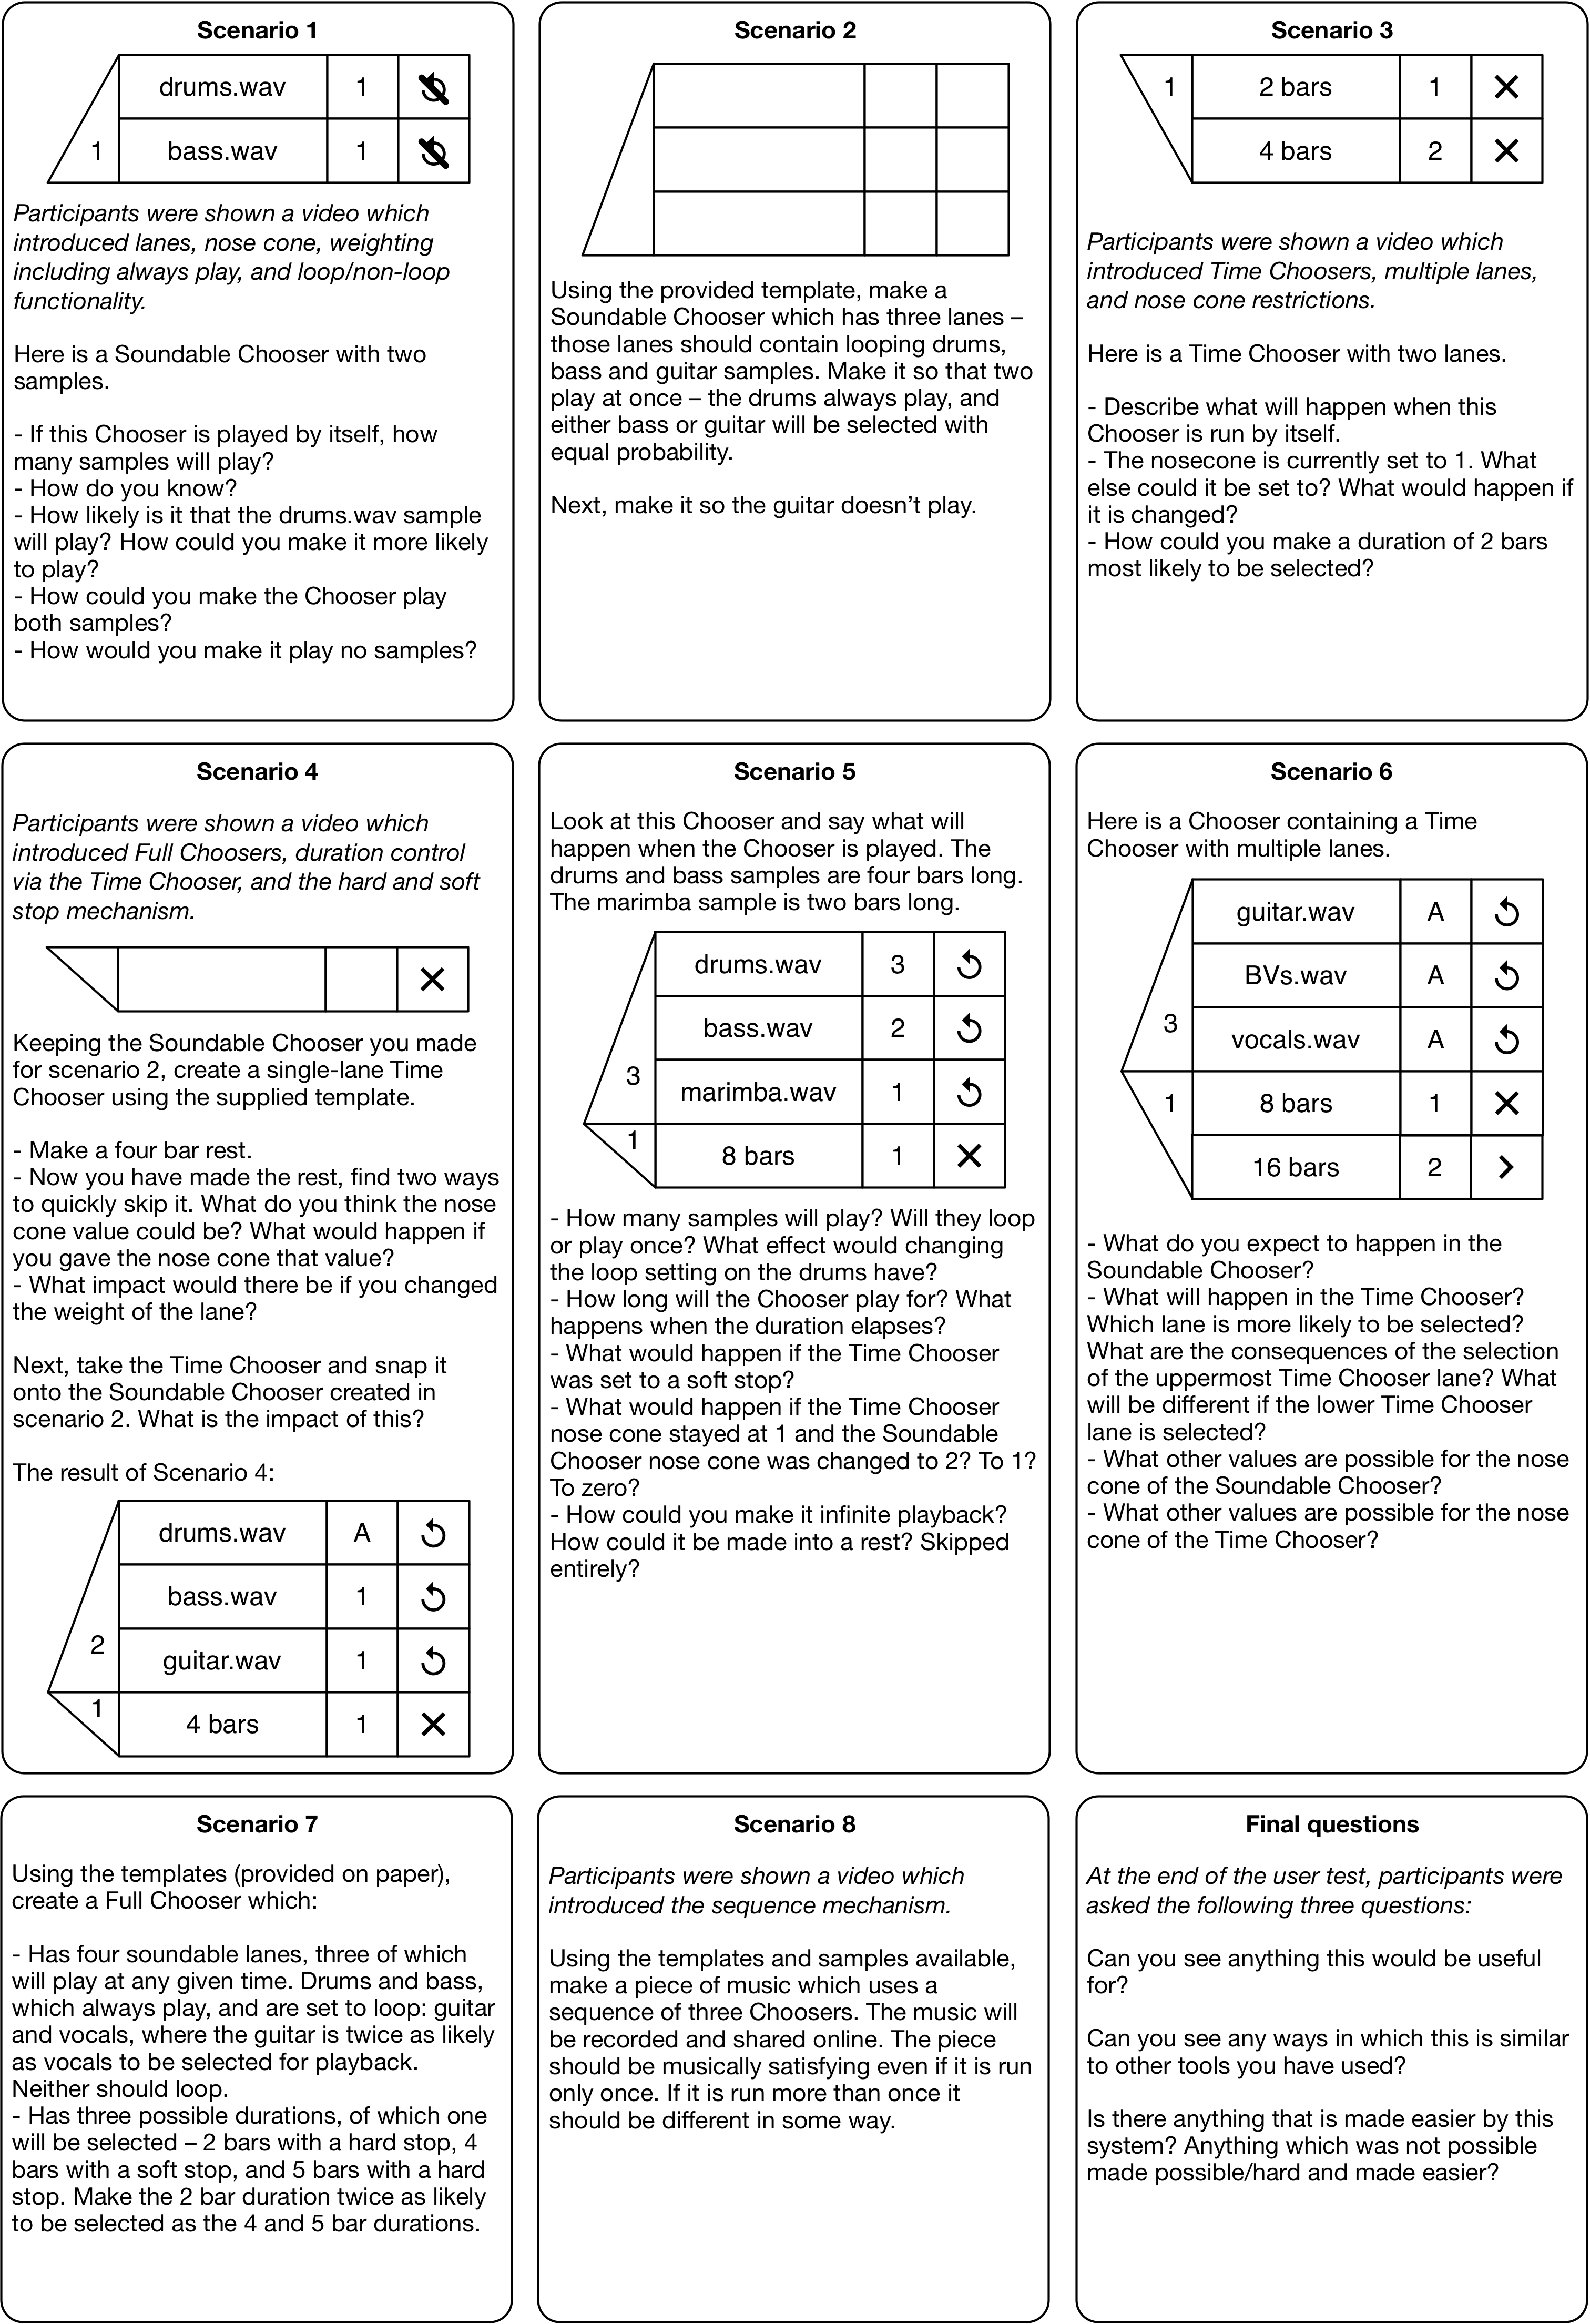
\includegraphics{./media/image3.png}
\caption{The eight user test scenarios.}\label{fig:three}
}
\end{figure}

\hypertarget{results}{%
\subsection{Results}\label{results}}

All participants were able to understand the behaviour of Soundable
Choosers. Twice participants had to be corrected after believing
vertically stacked lanes all play concurrently -- both instances of this
misunderstanding occurred in the first scenario only. Two groups found
multiple vertically aligned time lanes confusing and assumed that both
durations would play together, or one would play before the other. The
initial introduction of a Time Chooser as a representing a rest, and
only later showing it constraining a Soundable Chooser's duration, was
confusing for four of the seven groups. Hard and soft stops were
understood, but seven of the fourteen participants asked for
clarification of the behaviour of the soft stop. Two pairs of
participants suggested alternatives for the hard and soft stop icons.
Two participants wanted to use `always play' to express infinite
playback rather than removing the Time Chooser. There was some confusion
over the meaning of `always play' and whether it could be skipped. Some
felt the interface used numbers for too many parameters.

Three groups commented on the `boring' design. The layout of Choosers
was not seen as problematic, but some users wished for a more stylish
and polished presentation. Two groups requested colours to enhance
usability: within one group, one user wanted automatic colour selection
(denoting lane type) and the other user felt that user-controlled colour
selection would better support sorting and arrangement tasks. Several
users were interested to know if lanes could be rearranged to visually
organise lanes into instrument groups. One user suggested that lane
arrangement could be an alternative to the weight column --- moving a
lane higher would result in a higher probability of playback. This is
similar to one mechanism which was considered and rejected before the
user tests: it was replaced by the weight column as the column allows
for multiple identical lane weights, quick auditioning, and
user-controlled lane ordering to assist with musical arrangement. One
user requested instrument icons for lanes, partly in response to being
unaware of the marimba (one of the samples used in the user test).

Overall, participants were able to complete all scenario tasks, with
varying levels of assistance.

\begin{figure}
\hypertarget{fig:four}{%
\centering
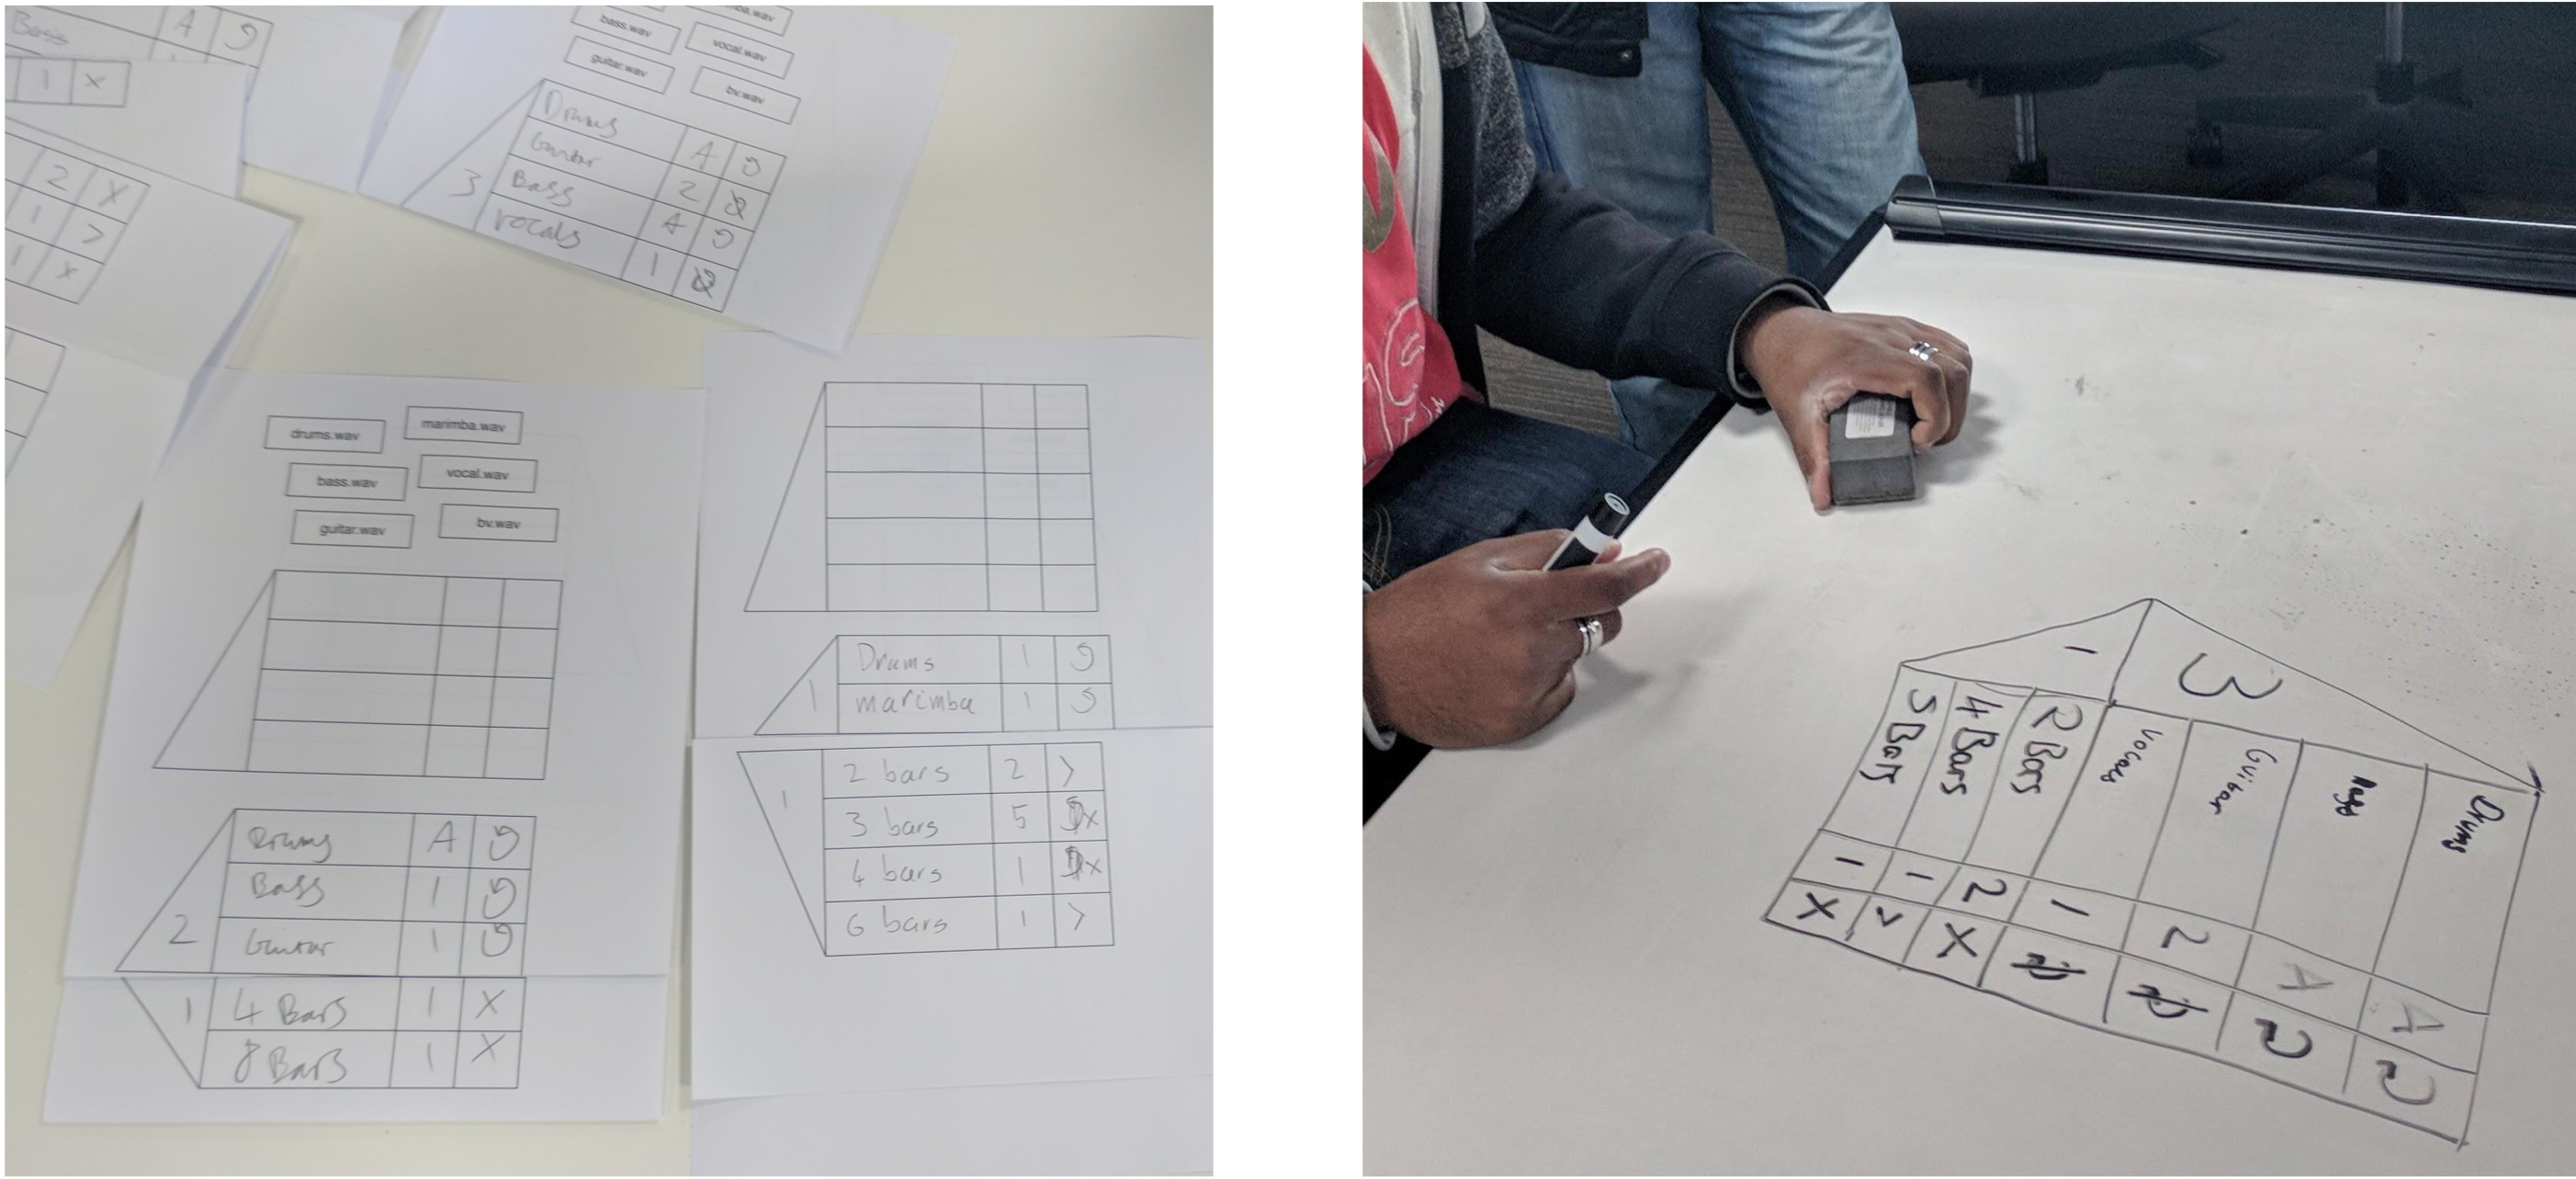
\includegraphics{./media/image4.png}
\caption{User work on paper and on a whiteboard.}\label{fig:four}
}
\end{figure}

\hypertarget{reflection-on-design-issues}{%
\section{Reflection on design
issues}\label{reflection-on-design-issues}}

The findings from the user tests outlined above have various
implications for the design of Choosers.

\hypertarget{sec:musicalissues}{%
\subsection{Musical issues}\label{sec:musicalissues}}

Repeating phrases, and the musical interaction between phrases, are
crucially important in a music system. These have therefore been brought
to the surface via the loop and hard/soft stop behaviours. We found that
the stop behaviour was confusing to four of the seven pairs of users,
and the documentation will be enhanced to better explain the system. The
hard and soft stop system can be conceptualised in a number of ways. For
musicians, one useful way is to consider soft stops as suitable for
melodies, and hard stops for accompaniment. Melodies are therefore
allowed to finish, whereas accompanying elements are stopped when the
duration of the Chooser elapses.

Three of the fourteen users were keen to have a visual indication of
current position with respect to duration, such as a progress bar. While
this seems a reasonable request, it is complicated by the
non-deterministic nature of the system.

A significant number of participants found the use of Time Choosers for
both rests and Chooser duration to be confusing. This was largely due to
rests being introduced before the Time Chooser's primary function, which
is to control the duration of a Chooser.

None of the participants had experience in algorithmic composition, so
these sessions essentially introduced algorithmic compositional tools
while also testing the interface. This led some participants to presume
that the concepts themselves were novel. Some time was spent discussing
the desirability of algorithmic processes rather than this specific
implementation. Two participants assumed that the process would lead to
a linear audio file, which indeed it can, but many use cases would
require the music to remain nonlinear. Future evaluations could explore
the nature of attitudes to nonlinear playback, including how it is
related to expectations set by commercial music creation software and
linear playback. We are also interested in the use of Choosers in genres
which routinely incorporate extemporaneous changes and improvisation,
such as folk and jazz.

One group specifically wanted a mechanism to allow them to easily reuse
material for thematic development. The design of Choosers allows for
this via the nesting of Choosers within lanes, although it was not
included in the user tests for simplicity. The users were shown nesting
in response to their questions and found it to meet the need they had
expressed.

Choosers can be used in the creation of a range of music. However, given
the unusual combination of usability and affordances, Choosers are
particularly suited to music in which users would benefit from easy
access to non-linear playback. Some classic Minimalism techniques
{[}@Potter2002-nr{]}, such as phasing {[}@Scherzinger2005-ui{]}, are
easily achievable using Choosers. Game music is often non-linear,
created using layers of musical material which are triggered by in-game
events {[}@Collins2008-ua{]}. Such material can be created using
Choosers, and we have a mechanism which would allow for external input
via OSC or an alternative protocol; this would allow a game engine to
trigger changes in the music. Choosers also allow musicians and music
producers to create nonlinear versions of existing recordings by loading
alternate takes into Choosers. The playback could range from very close
to the original (e.g.~algorithmically switching between vocal takes of
the same melody) to playing significantly different material
(e.g.~branching to play different sections), depending on the decisions
made by the creators.

\hypertarget{programming-related-issues}{%
\subsection{Programming-related
issues}\label{programming-related-issues}}

As shown in @sec:system, the Soundable Chooser nose cone slopes down and
the Time Chooser nose cone slopes up -- this allows them to be joined
together and communicates the required upper/lower order to the user.
Interestingly, some users guessed the combination of Soundable and Time
Choosers, suggesting that the nose cone shapes of the two Chooser types
were effective in communicating their combinatorial usage.

The Chooser system is designed to allow for consistent logic to be
applied across Soundable and Time Choosers where possible. Participants
in the user tests successfully reused elements of the Soundable Chooser
system when manipulating duration, but there were some cases where such
reuse or re-contextualisation was not possible. Interestingly, the
actions of the users in these cases would have made sense neither from a
musical nor programming perspective, but the rationale behind these
requests is instructive as it shows how users understand the tools in
the system. For example, in scenario five (@fig:three) two participants
wanted to use the `A' (always play) mechanism to set infinite playback
-- they wanted to override the set duration and had understood `A' to be
a global override control. In a similar example, one user wanted to be
able to loop a Time Chooser. If the system were to be changed to allow
for a set number of repeats, rather than an infinite loop, such a move
may be desirable.

Users will also require access to metadata -- for example, to check the
length of a sample loaded into a soundable lane in a Chooser. Such
metadata could be shown via a tooltip, accessed by hovering the mouse
over a lane.

\hypertarget{shared-and-existing-knowledge}{%
\subsection{Shared and existing
knowledge}\label{shared-and-existing-knowledge}}

One design motivation is to enable people to understand the system very
quickly. The Chooser design tacitly draws on a number of systems of
existing knowledge.

Some users wanted to be able to leverage their existing understanding of
DAW software and found it frustrating that they needed to learn new
paradigms for duration, synchronicity, and so on. This is an example of
technological framing {[}@Orlikowski1994-mi{]}. The knowledge gained by
using other music software can be useful, but it can also prove
problematic if the design of the software being learned is sufficiently
differentiated. As a result, there is much to be gained by following
standard design conventions where possible, as this maximises the user's
ability to reuse existing knowledge. One interesting example was seen in
scenario 6 (@fig:three), in which one pair of users learned the rules of
Choosers and then wanted to use the same rules elsewhere.

Technological framing, and the expectations set by the use of commercial
DAWs, may be an influence on user requests for a progress bar and the
conversations on the desirability of nonlinear vs.~linear playback that
took place during the user tests (as considered in @sec:musicalissues).

\hypertarget{metaphor}{%
\subsection{Metaphor}\label{metaphor}}

Interface metaphors are very common and can be useful in communicating
the roles of the software and setting realistic expectations when users
are familiar with the original interface. However, such metaphors can
become problematic if users are not familiar with the original
interface.

Related to technological framing is the assumption, ubiquitous in
Digital Audio Workstations, that signal flow and processing will be
applied using a mixing desk metaphor. Such virtual desks often make use
of skeuomorphism (such as the fader caps and rotary potentiometers in
Pro Tools), although some other designs have made graphical changes
while retaining the overall layout. As an example, Ardour's use of a
textured `strip' instead of a fader is still skeuomorphic as it makes
use of a ribbon controller metaphor but, in an attempt to improve mouse
control by increasing the size of the target, it does not follow the
traditional desk layout.

Given that DAWs are now capable of performing all mixdown tasks, and the
financial cost of consoles and outboard effects processors can be
prohibitive, many users learn in a virtual studio environment rather
than on hardware. Many DAWs were designed to mimic hardware in order to
leverage existing knowledge and ease the transition from hardware to
software. However, now most people are introduced to music production
via software, and many do not use hardware, there is an opportunity to
revisit some design assumptions.

Some users felt that the user interface was `boring', lacking the use of
colour, metaphor, and skeuomorphic design common in DAWs. This may be
another example of technological framing {[}@Orlikowski1994-mi{]}. We
can also consider the impact of metaphor in music software by making use
of the Cognitive Dimensions of Notations {[}@Green1996-gb{]}. Using this
framework, the closeness of mapping and role expressivity of a mixing
desk can be implied by making a software recreation look and function
like hardware.

Some users had difficulty understanding the outcome of hard and soft
stops in Choosers. The vast majority of music production software is
focussed on the creation of linear music, and the concept of `play until
finished' is rarely implemented. As a result, none of the user test
participants had encountered it, and did not have a frame of reference
for why it might be desirable. As a result, there is not a clear
existing metaphor for what we refer to here as a `soft' stop. Users
agreed that the \(\times\) icon represented a traffic stop sign and that
it was a suitable analogy for `stop now', but the \(>\) icon used for a
soft stop was not immediately understood as there is no readily
accessible metaphor.

\hypertarget{sec:arithmetic}{%
\subsection{Arithmetic}\label{sec:arithmetic}}

The use of numbers and arithmetic relationships in an interface can be a
valuable organising tool, as they are more or less universally familiar
and can concisely represent many relationships. The decision to use
numbers for several parameters was motivated by parsimony and
consistency. However, the use of numbers for multiple parameters was
perceived as negative by three participants. Upon questioning, the issue
was that numbers meant different things in different parts of the
interface. The Chooser design presented to participants in the user
tests made use of integers in five different ways: for the number of
simultaneously playing soundable elements, weight, duration, repeats,
and Time Chooser on/off. Despite this, for different reasons, the user
issues surrounding the `always play' option led us to consider extending
the range of numerical concepts used in the interface, by allowing the
metaphorical use of \(\infty\) as a weight (to outrank any positive
integer weight) as discussed in the next section.

In @sec:solutions, we propose changes to Chooser design to address these
various issues.

\hypertarget{sec:solutions}{%
\section{Design problems and candidate solutions in
Choosers}\label{sec:solutions}}

Given the problems for some users with the use of integers for multiple
parameters (see @sec:arithmetic), we propose the use of a simple on/off
icon for the Time Chooser nose cone. Interestingly, one pair of users
suggested this change in the user tests. Scenario five (@fig:three)
showed that two users wanted to leverage the `always play' mechanism
beyond the weight column, and one user wanted to set the duration of a
time lane to infinity. We propose a change to Choosers which allows for
both mechanisms.

We propose a design change which allows the user to allocate a maximum
possible weight (\(\infty\))~for a lane, thereby guaranteeing that it
will play if the nose cone number is high enough to allow all such lanes
to play. When allowing \(\infty\) as a weight, a useful metaphor is to
think of lanes with weight \(\infty\) as having paid for `priority
boarding', as when boarding an aircraft. Lanes with weight \(\infty\)
will always be chosen before any lanes with any finite weight. Compared
with the `always play' mechanism, this has the potential for greater
clarity when the number of maximally-weighted lanes exceeds the number
of the nose cone. In such cases, under the current `always play' system
it is not obvious whether `always play' should override the nose cone or
vice versa. Under the proposed system, the nose cone would determine the
number of lanes to play, and if that was less than the number of lanes
with weight \(\infty\), the winners would be chosen from those lanes at
random. We are also considering the use of a maximum value (\(\infty)\)
for the nose cone of a Soundable Chooser (`play all available lanes')
and for the duration of a time lane (`play forever').

We propose that future work will introduce Time Choosers in the context
of a Full Chooser, with the rest functionality introduced later as a
special case. Tutorial materials will provide a clear explanation and
will offer context and examples. The value of all of these proposed
changes will be tested empirically.

\hypertarget{conclusions}{%
\section{Conclusions}\label{conclusions}}

Choosers were developed to allow non-programmers access to algorithmic
composition tools and processes. The design principles were to leverage
parsimony in order to enhance learnability; to surface musically
meaningful actions, and to make them quick and easy; to allow both
bottom-up and top-down construction; and to make use of progressive
disclosure to allow for advanced use without harming usability for
beginners.

The user tests outlined here show that non-programmers were able to
successfully use Choosers to create a number of short pieces of music.
Future work will focus on the refinement and re-evaluation of the
Chooser notation and supporting materials.

\end{document}
